% !TEX root = ../ac_paper.tex

\section{Introduction\label{sec:intro}}

\TBW

\subsection*{Outline}




This paper is structured as follows. In \autoref{sec:AC}, we review the Andrews--Curtis conjecture. In \autoref{sec:search}, we use classical search algorithms to study the presentations of Miller--Schupp series. We devise a greedy search algorithm and show that it performs significantly better than the breadth-first search algorithm widely used to study this problem in the literature. We discover that the previously-known shortest potential counterexample to the stable AC conjecture, i.e. $\AK(3)$, is in fact stably AC-trivial.

In \autoref{sec:rl}, we use reinforcement learning to search through the space of balanced presentations. Specifically, we focus on the Proximal Policy Optimization algorithm. We find that while this algorithm performs significantly better than breadth-first search, it does not outperform greedy search. (See \autoref{fig:performance}.)

In \autoref{sec:lm}, we use a decoder-only Transformer model to study the language structure of balanced presentations. We find that easy and hard presentations form their own clusters inside the embedding space of the Transformer model.

\begin{figure}
	\centering
	\begin{subfigure}[b]{0.5\textwidth}
		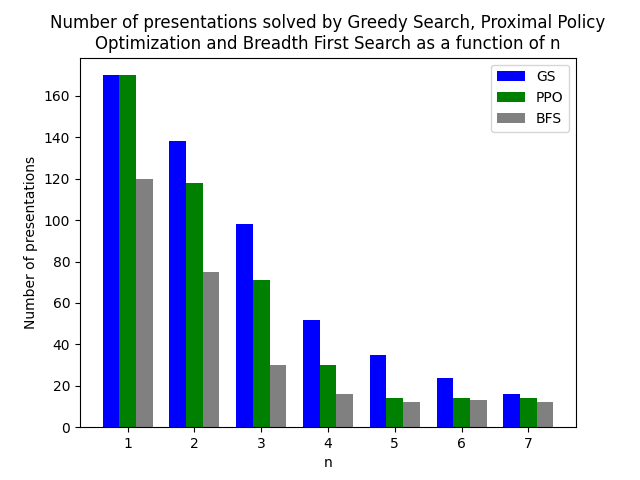
\includegraphics[width=1.1\textwidth]{fig/performance_vs_n.png}
		\caption{Distribution versus $n$}
		\label{fig:performance_vs_n}
	\end{subfigure}
	\begin{subfigure}[b]{0.5\textwidth}
		\centering
		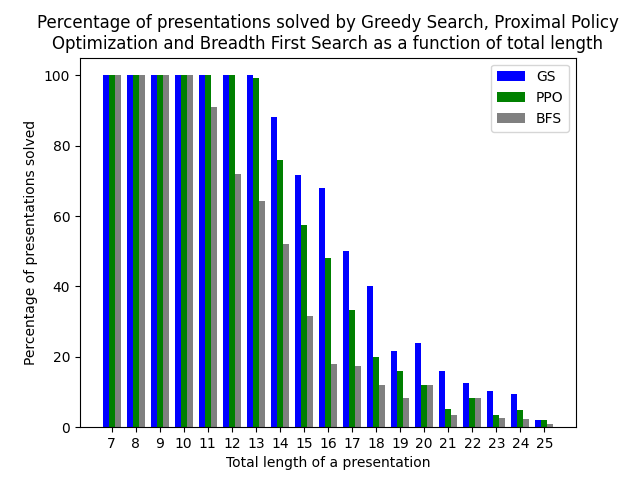
\includegraphics[width=1.1\textwidth]{fig/performance_vs_length.png}
		\caption{Distribution versus length}
		\label{fig:performance_vs_length}
	\end{subfigure}
	\caption{The figure shows a comparison of three algorithms --- breadth-first search, greedy search, and Proximal Policy Optimization (PPO) --- that we used to search through the space of balanced presentations. The number of presentations of the Miller--Schupp series, $\MS(n, w)$, solved by an algorithm is given on the vertical axis. We compare the performance as a function of $n$ (above) and the length of the presentation (below). Greedy Search consistently outperforms Breadth-First Search and Proximal Policy Optimization.}
	\label{fig:performance}\anibal{It would be better to include a PDF version of this pictures instead of a (compressed) PNG.}
\end{figure}

%We compare the performance of Greedy Search (GS), Breadth First Search and Proximal Policy Optimization on the presentations of Miller--Schupp series with $n, \ \length(w) \leq 7$ in \autoref{fig:performance}.
